% Draft for the Springer Nature "Code&Data in Earth Science" call.
% Structured for the official Frontiers of Computer Science (FCS) LaTeX template.
% Compile with the fcs.cls and companion files from the FCS 2026 template ZIP.
% Complete all bracketed author/declaration fields before submission.
\documentclass[review]{fcs}
\usepackage{tikz}
\usetikzlibrary{positioning}

\title{SciGeoGuard-X: Evidence-Carrying Verification and Conservative Repair for Earth-Observation Workflows}
\author*[1]{[Author name]}
\address[1]{[Department, institution, city, country]}
\fcssetup{corr-email = {[corresponding author email]}}
\keywords{Earth observation, workflow verification, geospatial software, provenance, scientific reproducibility}

\begin{document}
\maketitle

\section{Software description}
Earth-observation workflows can run without errors yet violate the scientific meaning of their inputs or outputs. SciGeoGuard-X is an open-source Python tool that checks workflow descriptions against explicit scientific intent and metadata, reports evidence-linked findings, and proposes conservative repairs only when required evidence is present. The v11 EarthRefine layer organizes findings as named refinement obligations, emits machine-readable certificates, and re-verifies candidate repairs.

The tool represents artifacts, processing steps, and analysis intent as Python objects. An \texttt{Artifact} can record quantity, unit, spatial and temporal resolution, coordinate reference system (CRS), processing level, acquisition and availability times, provenance, measurement scale, and domain attributes. A \texttt{Step} describes an operation such as resampling, temporal aggregation, index calculation, or model evaluation. An \texttt{Intent} records the requested quantity, unit, time, spatial support, quality constraints, or physical range. The \texttt{verify\_science(artifacts, steps, intent)} function returns \texttt{PROVEN}, \texttt{REFUTED}, or \texttt{UNPROVEN}; each finding contains a diagnostic code and evidence. These verdicts apply only to the implemented checks and supplied metadata.

The v11 layer groups diagnostics under named obligations. \texttt{evidence\_certificate} serializes findings with a hash of the described workflow; the hash identifies the input description and does not certify source data. \texttt{synthesize\_minimal\_repair} searches a bounded set of one- or two-edit candidates and accepts one only if the same verifier returns \texttt{PROVEN} after rechecking. It does not create missing observations or establish suitability beyond encoded rules. Users can install the repository and run \texttt{python examples/quickstart.py}; the v11 notebook reproduces the repair experiment. Source, tests, examples, notebooks, and frozen result files are available in the public repository \cite{sgg}.

\section{Earth-science use}
NASA documents IMERG precipitation products in rate units such as mm h$^{-1}$ and distinguishes rates from accumulations in mm \cite{imerg}. A half-hourly rate cannot be summed directly and interpreted as a depth; the rate must be integrated over the sample duration. A user can describe an IMERG rate artifact with unit \texttt{mm/hr} and temporal resolution 0.5 h, then describe an aggregation that requests accumulation in mm. If the operation sums rates without duration weighting, SciGeoGuard-X reports \texttt{RATE\_SUM\_WITHOUT\_DURATION} or \texttt{RATE\_AVERAGED\_AS\_ACCUMULATION}, depending on the operation. When sample duration is declared, the repair layer can propose duration-weighted integration and rerun the checks. This is a metadata-level usage example; it is not a new analysis of IMERG observations or an independent validation of rainfall estimates.

\section{Evaluation and limitations}
In controlled author-generated tests, v11 detected 10/10 designed semantic mutations. A safe one-edit repair was found for 9/10 mutation families, and all 9 found repairs re-verified. On a frozen set of 180 generated-reference cases, the tool agreed with all stored labels; among 112 cases labeled \texttt{REFUTED}, 47 received a conservative one-edit repair and all 47 re-verified. The labels and mutations were generated or controlled by the project authors. These counts measure consistency with encoded rules, not independent scientific accuracy, sensitivity, specificity, or field performance. Rule coverage is incomplete, and incorrect or missing metadata can mislead. A separate blinded review is incomplete and is not included.

\section{Availability and maintenance}
SciGeoGuard-X is available at \url{https://github.com/bnssaanirudh/SciGeoGuard} \cite{sgg}. The authors must confirm the release to cite and maintain resource availability for at least two years after publication, including a link to the published paper, as required by the call.

The verification and conditional repair sequence is summarized in Fig.~\ref{fig:workflow}.

\begin{figure}[!ht]
\centering
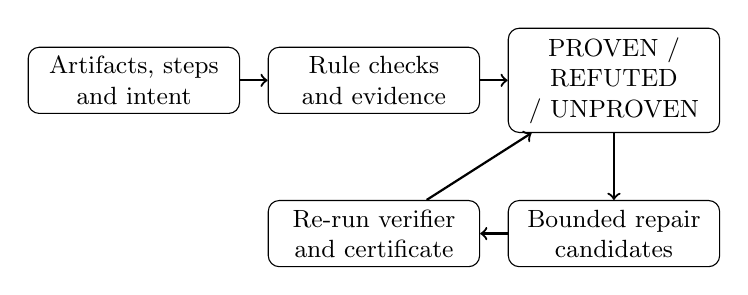
\begin{tikzpicture}[node distance=0.35cm, every node/.style={draw, rounded corners, align=center, minimum height=0.75cm, text width=2.45cm, font=\small}, arr/.style={->, thick}]
\node (in) {Artifacts, steps\\and intent};
\node[right=of in] (check) {Rule checks\\and evidence};
\node[right=of check] (verdict) {PROVEN / REFUTED\\/ UNPROVEN};
\node[below=0.85cm of verdict] (repair) {Bounded repair\\candidates};
\node[left=of repair] (again) {Re-run verifier\\and certificate};
\draw[arr] (in)--(check);
\draw[arr] (check)--(verdict);
\draw[arr] (verdict)--(repair);
\draw[arr] (repair)--(again);
\draw[arr] (again)--(verdict);
\end{tikzpicture}
\caption{SciGeoGuard-X workflow. Repair is conditional; each candidate must pass the same encoded checks when re-verified.}
\label{fig:workflow}
\end{figure}

\begin{acknowledgement}
[Authors: complete funding, acknowledgements, and competing-interest statements.]
\end{acknowledgement}

\begin{thebibliography}{2}
\bibitem{sgg} SciGeoGuard-X contributors. SciGeoGuard-X source repository and reproducibility materials. \url{https://github.com/bnssaanirudh/SciGeoGuard}. Accessed 17 October 2026.
\bibitem{imerg} NASA Global Precipitation Measurement Mission. IMERG: Integrated Multi-satellitE Retrievals for GPM; product and technical documentation. \url{https://gpm.nasa.gov/data/imerg}. Accessed 17 October 2026.
\end{thebibliography}

\end{document}